\documentclass[11.5pt]{sig-alternate} % sets document style to sig-alternate
% packages
% typesetting
%\usepackage{dirtytalk} % typset quotations easier (\say{stuff})
\usepackage{hanging} % hanging paragraphs
\usepackage[defaultlines=3,all]{nowidow} % avoid widows
\usepackage[pdfpagelabels=false]{hyperref} % produce hypertext links, includes backref and nameref
\usepackage{xurl} % defines url linebreaks, loads url package
\usepackage{microtype}
\usepackage{textgreek}
%\usepackage{textcomp}
%\newcommand{\texttildemid}{\raisebox{0.4ex}{\texttildelow}}
% layout
\usepackage{enumitem} % control layout of itemize, enumerate, description
\usepackage{fancyhdr} % control page headers and footers
\usepackage{float} % improved interface for floating objects
%\usepackage{multicol} % intermix single and multiple column pages
% language
\usepackage[utf8]{inputenc} % accept different input encodings
\usepackage[english]{babel} % multilanguage support
% misc
\usepackage{graphicx} % builds upon graphics package, \includegraphics
%\usepackage{lastpage} % reference number of pages
%\usepackage{comment} % exclude portions of text (?)
\usepackage{xcolor} % color extensions
\usepackage[backend=biber, style=apa]{biblatex} % sophisticated bibliographies % necessary for HTML to display author info and date on abstract page
\usepackage{csquotes} % advanced quotations, makes biblatex happy
\usepackage{authblk} % support for footnote style author/affiliation
% tables and figures
\usepackage{tabularray}
%\usepackage{array} % extend array and tabular environments
\usepackage{caption} % customize captions in figures and tables (rotating captions, sideways captions, etc)
%\usepackage{cuted} % allow mixing of \onecolumn and \twocolumn on same page
\usepackage{multirow} % create tabular cells spanning multiple rows
%\usepackage{subfigure} % deprecated, support for manipulation of small figures
%\usepackage{tabularx} % extension of tabular with column designator "x", creates paragraph-like column whose width automatically expands
%\usepackage{wrapfig} % allows figures or tables to have text wrapped around them
%\usepackage{booktabs} % better rules
% dummy text
%\usepackage{blindtext} % blind text dummy text
%\usepackage{kantlipsum} % Kant style dummy text
\usepackage{lipsum} %lorem ipsum dummy text
% other helpful packages may be booktabs, longtable, longtabu, microtype

\pagestyle{fancy} % sets pagestyle to fancy for fancy headers and footers

% header and footer
% modern way to set header image
\renewcommand{\headrulewidth}{0pt} % defines thickness of line under header
\renewcommand{\footrulewidth}{0pt} % defines thickness of line above header
\setlength\headheight{80.0pt} % sets height between top margin and header image, effectively moves page contents down
\addtolength{\textheight}{-80.0pt} % seems to affect the lower height. maybe only works properly if footer numbers enabled?
\fancyhf{}
\fancyhead[CE, CO]{
\includegraphics[width=\textwidth]{headerImage.png}}
% footer
%\fancyfoot[LE,LO]{Article Title Here \\ DOI: }% left footer article title and doi
%\fancyfoot[CE,CO]{{}} % center footer empty
%\fancyfoot[RE,RO]{\thepage} % right footer page numbers
%\pagenumbering{arabic} % arabic (1, 2, 3) numbering in footer

\hypersetup{colorlinks=true,urlcolor=blue} % sets link color to blue
\urlstyle{same} % sets url typeface to same as rest of text

% set caption and figure to italics, label bold, left align captions, does not transfer to HTML
\captionsetup{labelfont=bf, font={large, it}, justification=raggedright, singlelinecheck=false}
\renewcommand\theContinuedFloat{\alph{ContinuedFloat}}

%this next bit is confusing, but essentially changes the width of the abstract. Seems to have been copied from this https://tex.stackexchange.com/questions/151583/how-to-adjust-the-width-of-abstract
\let\oldabstract\abstract
\let\oldendabstract\endabstract
\makeatletter %changes @ catcode to enable modification (in parsep)
\renewenvironment{abstract} %alters the abstract environment
{\renewenvironment{quotation}%
               {\list{}{\addtolength{\leftmargin}{1em} % change this value to add or remove length to the the default ?
                        \listparindent 1.5em%
                        \itemindent    \listparindent%
                        \rightmargin   \leftmargin%
                        \parsep        \z@ \@plus\p@}%
                \item\relax}%
               {\endlist}%
\oldabstract}
{\oldendabstract}
\makeatother %changes @ catcode to disable modification

% checks
% italics
% links
% dashes
% tildes
\begin{document}

\title{Pedagogical Applications of Instant Messaging Technology for Deaf and Hard-of-Hearing Students in the Science Classroom}

\author[1]{\large \color{blue}Todd Pagano}
\author[1]{\large \color{blue}L.K. Quinsland}

\affil[1]{ Rochester Institute of Technology/National  Technical Institute for the Deaf}

\toappear{}
%% ABSTRACT
\maketitle
\begin{@twocolumnfalse} 
\begin{abstract}
\item 
\textit{For deaf and hard-of-hearing individuals, the emergence of Instant Messaging technology and digital pagers has been perhaps one of the greatest liberating communication technological breakthroughs since the advent of the TTY.  Instant Messaging has evolved into an everyday socially compelling, portable, and “real time” communication mode for students.  The focus of this paper is on the pedagogical implications of using Instant Messaging technology to promote student learning and on the process of implementing the technology in order to engage deaf and hard-of-hearing students, both in and out of the science classroom.  Applications include in-class learning activities (in homogeneous and heterogeneous communication mode classrooms), out-of-class discussion/study groups, “virtual lectures” with content experts in the field, and communication with students while on co-operative work assignments.  Perceived benefits to deaf students, deaf and hearing students in an inclusive environment, as well as benefits to teaching faculty are presented.  Technological modifications and instructional application protocols (i.e., hardware, software, and logistical considerations) that are required to maximize the student learning experience are also discussed. }
\\ \\
\end{abstract}
\end{@twocolumnfalse}

%% AUTHOR INFORMATION

\textbf{*Corresponding Author, Todd Pagano }\\
\href{mailto: tepnts@rit.edu }{(tepnts@rit.edu)} \\
\textit{Submitted  Apr 14 2014}\\
\textit{Accepted Apr 14 2014} \\
\textit{Published online Apr 14 2014} \\
\textit{DOI:10.14448/jsesd.01.0004} \\
\pagebreak
\clearpage
\begin{large}
\section*{INTRODUCTION}
A few years ago, for about the eleventh time that particular day, we had to remind one of our deaf students that text pagers, like cell phones in a restaurant, are not acceptable for use during class activities. Later in that period, the class took a brief break and the students rushed to the computers lining the back wall of our laboratory classroom, only to begin typing zealously. We observed the now familiar sight of Instant Messages (IM) popping up on the computer monitors from students’ extensive “buddy lists” (with the students entertaining several “chats” at one time). Instantaneously, what might be termed an educational epiphany from a teaching perspective occurred. Clearly, something very powerful, compelling, and motivating to our students had been happening right in front of our eyes. Every teacher yearns for that ``teachable moment'' that seems to spontaneously appear far too infrequently. This was ours. We decided to attempt to harness this tool and investigate the components of ``their'' technology that could be applied with deaf and hard-of-hearing (d/hh) students in the science classroom. 

The current group of college students, the “Millennial Student” (“Generation Text”, “Generation Y”, or whatever label might be placed on them), are accustomed to certain technology and have always existed in the “Information Superage”. The technologically enhanced life that they embrace is not necessarily the same one that most faculty have experienced. These students are internet savvy, younger than IM technology itself, and have always had the expectation of access to no-delay communication being “one click away”. 

IM is one such technological tool that is a mere everyday communication mechanism to our students, and something that has always been prominent during their lifetimes. America Online’s™ IM program (AIM™)-or its subsidiary; ICQ™ (pronounced “I see you”), Microsoft’s™ version (MSN Messenger™), Yahoo!’s™ Messenger, and Mac’s iChat™ are just a few of the more popular software/portals that students use to satisfy their IM needs. A 2005 report by the Pew Internet \& American Life Project estimates that 66\% of “Generation Y” internet users (people age 18-28)-typical college students-use IM compared to 38\% of “Trailing Boomers” (age 41-50) and 42\% of “Leading Boomers” (age 51-59)-who are about the age of typical college faculty (Fox, 2005). Today’s students often prefer IM over email for communication, have the technology on their mobile communication devices, and spend a staggering number of hours using IM. 

So why not use this tool with which students are so comfortable for educational purposes? Philip Long stated “If culture has moved to adopt technology in commerce, in industry, in recreation, and in daily life, higher education may be legitimately slow to react, but react it must” (Long, 2002). Many colleges/universities currently use IM as a means for students to communicate with library help desks, campus computing troubleshooting, and tutoring resources. In fact, a growing number of college/university admissions departments are using IM as a vehicle for prospective students to communicate with admissions counselors, with several institutions also moving into the trendy Facebook and MySpace realm for recruitment (Farrell, 2007). However, the purpose of this paper is to go a step further and discuss the specific use of IM for pedagogical applications. 

D/HH students are no different than their hearing peers in regard to their everyday use of technology. In fact, through the use of pagers and smartphones, these students may even be more dependant on text-to-text communication technology than the hearing student who relies on mobile cellular phones. In their report about making Information Technology accessible for d/hh individuals, Tom Peters and Lori Bell articulate a trend toward preference of IM over the TTY (Peters, 2006). Estimates vary for the number of IM messages that are sent annually, but in 2000, it was extrapolated that Americans sent 423 billion IMs per year (Duesterberg, 2000). IM usage has certainly grown since the turn of the millennium, and when combined with the staggering number of text messages that are sent via mobile devices, might that quantity reach the trillions today? In fact, it is interesting to note that text messaging has become such a norm that the authors receive automated text messages to their mobile phones when the fume hoods in the academic laboratories malfunction or drop below a threshold ventilation flow rate. Perhaps for the first time, d/hh students have achieved social communication equality with their hearing peers. 

For many years, educators have strived to implement traditional ``best practices'' in providing academic support for d/hh students. In addition, they have paid attention to emerging instructional technologies and have experimented with numerous classroom applications. This investigation into the utility of IM technology attempts to harness ``student social technology'' to better meet learning objectives. To this end, IM technology has successfully been taken into the educational realm. With this pedagogical tool comes teaching/learning benefits in applications with d/hh students in various types of learning environments and instructional contexts. 

\section*{HISTORY}
 
\subsection*{IM Technology}

IM is a relatively new application of computer communication technology. A Finnish student, Jarkko Oikarinen, invented an early relative of IM, internet relay chat (IRC), in 1988 (Park, 2006). In 1998, when America Online™ (AOL) acquired ICQ™ (which had recently filed for a patent on IM technology), the subsidiary had a membership of 11 to 12 million registered users-that membership grew to 135 million users (add that to AOL’s AIM™ 180 million registered users) when the patent was awarded in 2002 (Hu, 2002). Currently, IM is on the verge of becoming a key business communication tool. Ferris Research documented 10 million business IM users in 2002 and predicted 182 million business users by 2007 (Kontzer, 2003). Recently, JetBlue Airways™ announced that it will be experimenting with offering limited Wi-Fi service, including ability to use IM, on certain flights (Yu, 2007). 

IM users have developed their own “language”, with popular acronyms like \textbf{lol} (laughing out loud), \textbf{brb} (be right back), \textbf{ttyl} (talk to you later), and \textbf{idk} (I don’t know)-to name just a few. For a list of common IM acronyms, see \url{http://www.imacronyms.com/} (accessed December 24, 2007). In fact, the “Merriam-Webster Dictionary Word of the Year for 2007” is \textbf{w00t} –an IM or gaming word used to express joy (Merriam-Webster Dictionary, 2007). 

\subsection*{IM in Education}

The use of IM in educational setting seems to be trailing its popularity in the business world. In fact, the use of IM is often actively discouraged in academia. Steven Gilbert, President of the TLT Group™ stated ``When I visit a campus, most people never mention IM as one of the new instructional options. If they mention it at all, it's to ask about ways of PREVENTING students from using IM in public computer labs and in classrooms'' (Gilbert, 2003). In the same discussion, Trent Batson, Director of IITS at the University of Rhode Island and developer of an early internet communication pedagogical tool for d/hh students-the ENFI (English Natural Form Instruction) Project, stated ``Teachers are suspicious of things students like to do-the tendency is to deny them that instead of figuring out how to use that energy as teaching moments'' (Batson, 2003). In certain areas of natural fit, it seems that IM has begun to catch-on in higher education. IM has been used in distance learning courses (Hrastinski, 2006 \& Maushak, 2007) and used for “virtual office hours” (Wymer, 2006 \& Lih-Ching, 2006). Still, IM technology may be underutilized in classroom environments and for various other pedagogical applications. 

\subsection*{IM use by Deaf and Hard-of-Hearing Individuals}

Although studies are currently underway to develop the technology of, and to assess the effect on learning by, voice-to-text and live captioning technology (e.g., CART and C-print), there appears to be little effort expended on the investigation of IM as an alternative ``real time'' communication option. 

Frank Bowe reported in 2002 that 75\% of d/hh respondents reported using IM at home and 35\% reported using it at work (Bowe, 2002). In general, respondents reported that their IM use had significantly increased over the past few years and many reported using IM in “the same way hearing people use the phone” (Bowe, 2002). Some members of the deaf community believe that IM technology has worked to “level the playing field” and has proven to be a tool for equality (Felps, 2001). 

The power of IM to the deaf community was evidenced when the National Association of the Deaf (NAD) asked the FCC for IM open standards and interoperability (National Association of the Deaf, 2005). Deaflawyers.org lists IM and text messaging as communication options on their webpage and IM leader, AOL™, operates an ``Accessibility Help'' page for deaf consumers at \url{http://www.aol.com/accessibility/accessibility_help/deaf_and_hard_of_hearing.html} (accessed December 24, 2007). 

\subsection*{IM in the Education of Deaf and Hard-of-Hearing Students}

There is little work reported in the literature on the use of IM technology with d/hh students in an educational environment. To this end, this paper describes some of the early experimentation by the authors with IM technology in pedagogical applications for d/hh students. 

\section*{PEDAGOGICAL APPLICATIONS}

The authors have used networked laptop computers with IM technology to enhance student learning in the following homogeneous (all d/hh students) contexts: 1) facilitating group discussions; 2) facilitating review preparation for exams; 3) facilitating collaborative research in small groups; 4) facilitating out-of-class structured interactions and study sessions; 5) providing a mechanism for students to interact with topical experts and professionals at a distance (“virtual lectures”); and 6) providing a mechanism for faculty to follow-up with students on cooperative work (co-op or internship) assignments. In addition, we have assessed the feasibility of facilitating group discussions and review in a heterogeneous (mainstreamed) classroom environment. 

\subsection*{In-Class Discussion}

Numerous variations and applications of in-class IM activities are possible. Student “class chat groups” are a very effective tool for stimulating interactions and engaging students. These chats can be strategically developed and assigned by the instructor in order to meet a myriad of instructional objectives. For instance, an in-class IM chat activity might involve dividing a class into several distinct groups and assigning a problem to solve or a question to ponder. While each member contributes to the groups’ path toward completing the task at hand, the instructor can monitor the discussions and progress of all of the groups (as well as individuals) simultaneously by setting up all group chats screens/windows on the instructor’s computer. At any given moment, the instructor can participate in any of the group chats and provide additional information, clarification, lead the discussion onto a different path, or pose questions to the group or to individuals who seem to be holding back. At the conclusion of the session, the instructor can print a record of each group discussion, including the contributions of each participant. This printout can be a valuable record to the students in that group, an important resource to students in the other groups, and a documented feedback tool for the instructor to gauge the level of individual student comprehension of a particular topic/concept. 

\begin{figure*}[t]
    \centering
    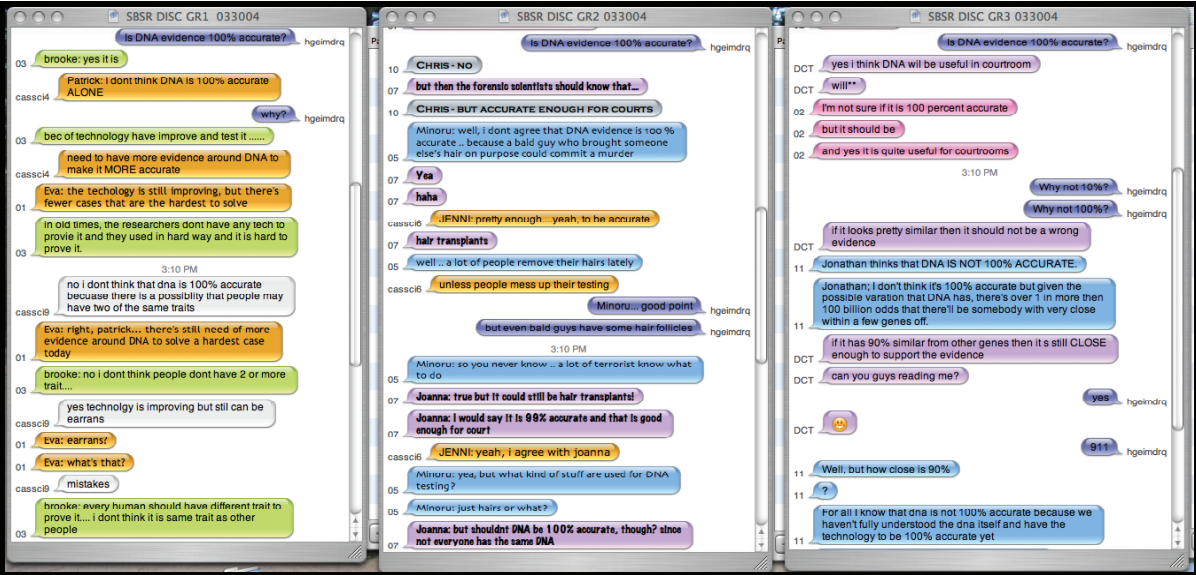
\includegraphics[width=1\textwidth]{images/fig1.png}
    \caption{Example In-Class Discussion IM Activity (the chat excerpt, using iChat™, shows the view from the instructor’s computer while monitoring several groups simultaneously). Note: student input is on the left side of each of the three screens while instructor input is on the right of each of the three screens. }
\end{figure*}

\subsection*{In-Class Review}

Review of concepts and processes occurs quite efficiently with the use of IM technology. Review questions can be prepared in advance (by the instructor or students) using a word processing program (i.e., Microsoft Word™) and subsequently pasted into the IM text box to facilitate rapid Question \& Answer (Q\&A) periods. Compared with traditional face-to-face Q\&A sessions, IM reviews can often take place in roughly half the time. Again, an additional benefit to the instructor is that the entire review can be printed, distributed, and analyzed. Students who demonstrated confusion, lack of preparation, or misunderstanding can then be approached and assisted individually. 

\begin{figure}[ht]
    \centering
    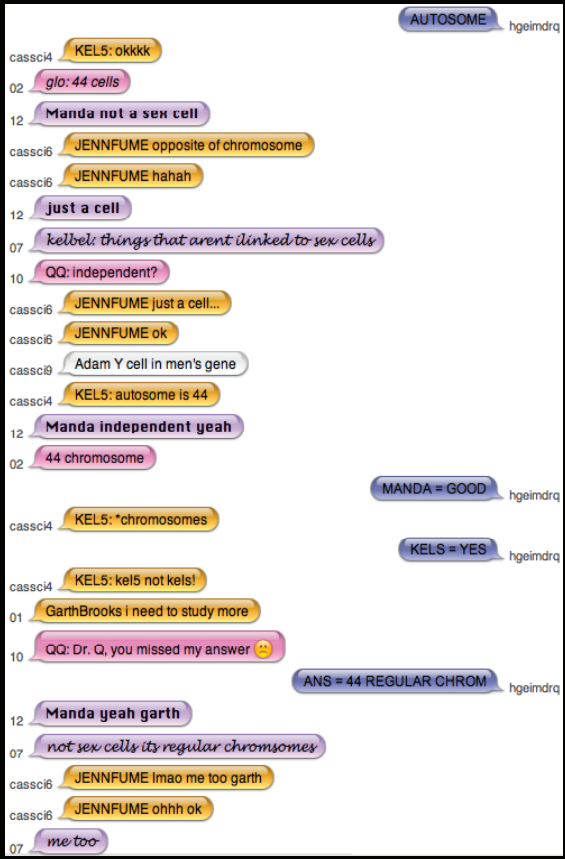
\includegraphics[width=0.85\linewidth]{images/fig2.png}
    \caption{Example In-Class Review IM Activity (the chat excerpt was pulled directly from iChat™). Note: again student input is on the left side of the screen while instructor input is on the right side of the screen.}
\end{figure}

\subsection*{In-Class Collaborative Research}

Students in small groups can be given a topic to research (e.g. thalidomide) as well as several ``starter'' questions. The group is told that all communication must be exclusively through typing via IM. Students are asked to each generate one more question to add to the researchable questions list. The goal of the activity is for the group to produce a research report that answers all of their questions, defines key vocabulary, and includes all citations in support of their findings. Students individually search for information, share information and citations with each other, and import text into a separate report summary document. Upon completion, all members of the group sign the research report. 

\begin{figure}[ht]
    \centering
    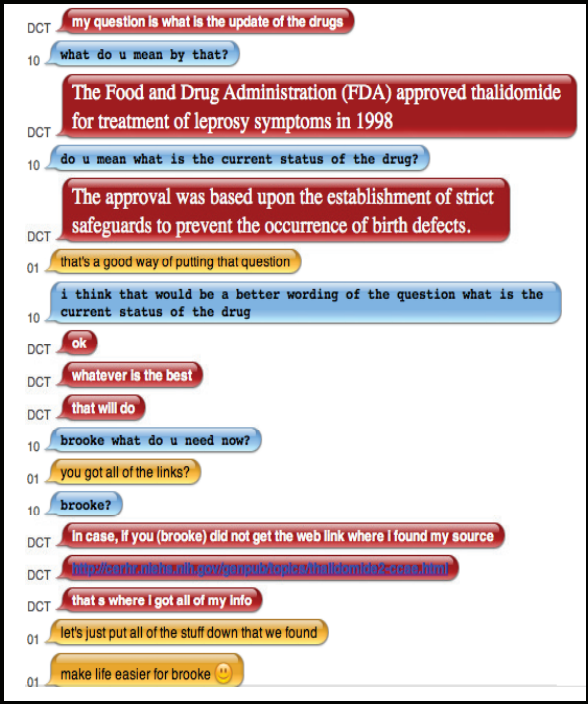
\includegraphics[width=0.9\linewidth]{images/fig3.png}
    \caption{Example Collaborative Research IM Activity (the chat excerpt was pulled directly from iChat™). Note: this portion of the chat is entirely between students. }
\end{figure}

\subsection*{Out-of-Class Interactions}

IM technology also creates a new mechanism for valuable out-of-class interactions. These activities allow course-related interactions (instructor-student and student-student) to occur during evening and weekend hours. Out-of-class discussions, or “Virtual office hours” (in the case of instructor-student communications), create a vehicle for “extending” learning opportunities while avoiding in-class time restrictions and establishing opportunities for continuous dialog. Out-of-class chat group assignments can be made for groups to convene online at specified times, including nights and/or weekends, and conduct class-related business. In effect, this activity serves as a type of “hyperspace/virtual study group”. The instructor can select and vary the group make-up when assigning group membership. Students can be taught how to configure their “class chat group” to fit the in-class or out-of-class assignment. 

\subsection*{Interactions with Topical Experts}

Using IM technology, students in classroom settings are able to interact with discipline-specific professionals and topical experts in the field. In a sense, these interactions act like “virtual lectures”. The information, coming directly from those working in the specific content area in which the students are concurrently learning in their academic courses, allows students to get timely, first hand, real-world, and “cutting edge” information. For example, a researcher in the pharmaceutical industry in California can participate in an IM chat (from the comforts of his/her office) with students in a classroom in New York related to an industry-specific spectroscopic technique that the students happen to be studying. The IM chat can again be printed and used to reinforce the material or placed into the course curriculum for future years. IM technology provides a mechanism for bringing educational experiences to the classroom that would otherwise be logistically prohibitive (e.g. finances, time constraints, or travel requirements). In addition, classroom communication can be difficult with outside experts/guest lecturers, who may not be familiar with d/hh communication protocol. In this case, the instructor can facilitate the text interaction between guest and students with a minimal need for paying attention to communication logistics. 

\begin{table}[htbp]
\begin{tabular}{|l|}
\hline
\textcolor{blue}{Student \#7}: What instruments do you use often at your job? \\
\textcolor{violet}{LST VISITOR}: Oh, I see them all...GC, GC-MS, different kinds of spectrophotometers (UV-Vis, IR), HPLC... \\
\textcolor{violet}{LST VISITOR}: Are you familiar with all of those? \\
\textcolor{cyan}{Student \#11}: Pretty much, yes \\
\textcolor{orange}{Student \#9}: we are going to learn how use them all \\
\textcolor{blue}{Student \#7}: We are studying UV-Vis Spectrophotometers now in our class \\
\textcolor{red}{Student \#12}: Is Beer’s Law really as important as our professor says? \\
\textcolor{violet}{LST VISITOR}: Beer’s Law is extremely important…the relationship between analyte concentration and absorbance is the reason we can extract the important information from the instruments.\\
\textcolor{violet}{LST VISITOR}: What do you guys study other than instrumentation? \\
\textcolor{green7}{Student \#1}: a lot on chemical analysis \\
\textcolor{orange}{Student \#9}: We study analytical chemistry- such as titrations, dilutions… \\
\textcolor{green7}{Student \#1}: chemical preparation \\
\textcolor{blue}{Student \#7}: a lot of hands on lab experimentation \\
\textcolor{violet}{LST VISITOR}: like what kinds of chemical analyses. specifically? \\
\textcolor{violet}{LST VISITOR}: volumetric? \\
\textcolor{red}{Student \#12}: Yes, titrations \\
\textcolor{violet}{LST VISITOR}: gravimetric? \\
\textcolor{green7}{Student \#1}: yes \\
\textcolor{red}{Student \#12}: both \\ \hline
\end{tabular}
\captionof{figure}{Example IM Chat with a Topical Expert (the chat excerpt was pulled directly from AIM™). Pedagogical Applications of IM}
\end{table}

\begin{figure}[!h]
    \centering
    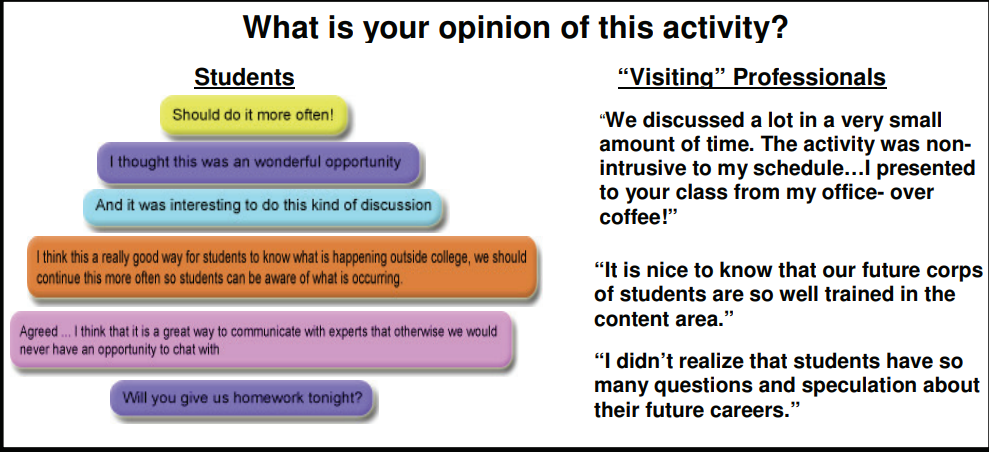
\includegraphics[width=1\linewidth]{images/fig5.png}
    \caption{Select Student and “Visiting” Professionals Opinions of IM Activity (the student responses were pulled directly from iChat™). }
\end{figure}

\subsection*{Co-op/Internship Progress Chats }

Though specific to postsecondary programs that allow for students to perform cooperative work experiences (co-ops) or internships, IM has pro-ven to be a very useful tool for monitoring student performance while on their work assignments. A quality co-op/internship can be mutually beneficial to the student and host workplace. Likewise, as most collegiate programs strive to keep good relations with their industrial partners, it is vital that the student co-op/internship process runs smoothly. To this end, IM has been used to “check-in” with students during their co-ops/internship, make sure that the experience is being a positive part of their educational program, discuss technical issues that have come up and might need reinforcing, discuss how to deal with behavioral and social issues that might arise with coworkers, and process how information that students have learned in prior coursework is being applied in their work assignment (a connection that is not always obvious to students). 

To avoid interrupting the workday, coop/internship IM interactions do not occur during typical work hours, but rather in the evenings during the work week. A group of students who are simultaneously completing their co-ops/internships are directed to all sign onto IM at a specific time (i.e., 8pm EST on Thursdays). It is important to note that since students may be working independently on opposite coasts of the country, a time must be chosen that is logistically practical for students in all time zones. Typically, one faculty member monitors an approximate hour IM chat with a group of about four students. These chats occur at the same time each week throughout the duration of their work assignments. A major benefit of having group chats is that it allows students to interact with each other and learn from others’ experiences. This peer learning outcome is manifested in the fact that several students are likely to have the same struggles in their respective assignments. As well, students have the opportunity to learn what workplaces other than their own are like, and can gain a more macroscopic vision of what their future career might be like. 

As is the case with all of the IM applications discussed here, a script of the chat can be printed and used for a variety of pedagogical purposes. We have found that IM used in this way can greatly improve student coop/internship experiences. It can serve as an early intervention tool for issues that arise (technical and social), an enjoyable mechanism for classmates who have been distanced for a period of time to “reconnect”, and a far more dynamic means of processing information than the typical method of students keeping a daily and static journal of their experiences. 

\begin{table}[htbp]
\begin{tabular}{|l|}
\hline
\textcolor{blue}{Co-opStudent\#1}: \textbf{For micropipette use, my company is very particular about it} \\
\textcolor{red}{Professor}: I’m not surprised. Please tell us about their technique. \\
\textcolor{blue}{Co-opStudent\#1}: \textbf{They have said that the micropipette must be standing upright, not angled. And before you use it for analytical purposes, you must check its calibration using the analytical balance} \\
\textcolor{blue}{Co-opStudent\#1}: \textbf{…using distilled water} \\
\textcolor{green7}{Co-opStudent\#2}: Interesting. Micropipettes are also important where I work. However, we calibrate using a special spectrophotometer \\
\textcolor{red}{Professor}: Congratulations, you have both hit on the two main ways to calibrate a micropipet \\
\textcolor{blue}{Co-opStudent\#1}: \textbf{yeah, it’s good to know that it is working properly} \\
\textcolor{red}{Professor}: we should add that activity to the LA II Quality Control course in the program. \\
\textcolor{green7}{Co-opStudent\#2}: I agree \\ \hline
\end{tabular}
\captionof{figure}{Example Co-op/Internship IM Chat (the chat excerpt was pulled directly from AIM™).}
\end{table}

\subsection*{In-Class Review (Mainstreamed Classroom)}

As with most innovation, experimentation leads to expanded insight. It soon became apparent that applications of IM technology in the classroom could easily transcend the homogeneous (all d/hh students) classroom and might have implications for attempting to level the playing field for d/hh students in the heterogeneous (d/hh/hearing students) mainstreamed classroom. D/HH students matriculated in colleges and universities are often marginalized in the mainstreamed classroom due to communication restrictions. While teacher-centered lectures, with limited student interaction, tend to function effectively with traditional support by sign interpreters and CPrint/CART (Communication Access Real-time Translation), IM applications allow for greater involvement of d/hh students in certain mainstreamed classroom activities. Attempts to utilize cooperative group learning strategies with d/hh and hearing students using traditional direct managed sign communication and/or interpreting support tends to limit spontaneous interactions due to inherent communication pacing issues or the ``lag time'' required to bridge signed and spoken communication. 

Tested examples of using IM in mainstreamed class environments include small group discussions and exam review sessions. In instances where the goal is for d/hh students to be truly involved in discussions with other students, if given a topic, students can immediately begin keyboarding without waiting for the interpreter-centered communication circle to be formed. The recommended mixture is four d/hh and hearing students per group, each student using a laptop that is linked to the other three members in the group using a chat network. Students report that this application of IM technology makes them feel like equal contributors, and therefore, learning partners with the hearing students in the class. 

In some types of mainstreamed activities, we have had success substituting a ``keyboarding facilitator'' for the traditional sign interpreter. A traditional exam review in a mainstreamed classroom setting, for the most part, excludes the d/hh student from participation due to the inherent “lag time” of sign interpreting or C-Print/CART. By the time the instructor speaks the question and the d/hh student receives that question, the instructor has often already acknowledged a spoken answer from a hearing student in the class and has moved on to the next question. In one trial, two deaf and two hearing students were given laptops. The keyboarding facilitator rapidly typed each review question and then voiced all student responses from the IM medium. The instructor added facilitator voiced responses to those obtained from hearing students in the class as he rapidly listed correct responses on a white board. Two remarkable outcomes were noted: 1. Approximately 50\% of the listed responses came from the group of four using the IM technology; and 2. The deaf students stated that this was the first time they felt like equal contributors to the class. 

Since adding an additional keyboarding facilitator to the interpreting support staff in a classroom is not necessarily economically feasible, it appears that we may have discovered a very successful instructional application of IM without an easy means of delivery. With this in mind, the interpreters present were asked their opinion of the activity. Both stated that they could not see the advantage over what they would normally do and stated that they could not envision adding keyboarding to their job description. 

\begin{figure}[!h]
    \centering
    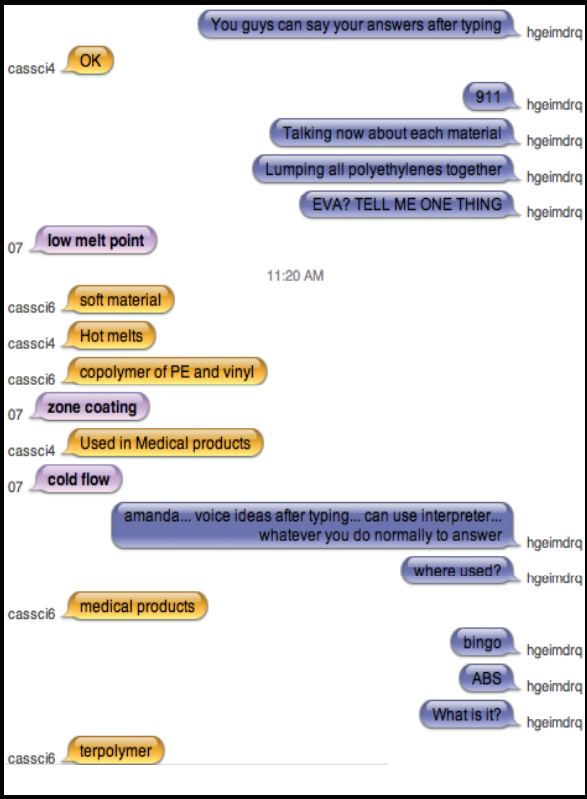
\includegraphics[width=1\linewidth]{images/fig7.png}
    \caption{Example In-Class Review (Mainstreamed Classroom) IM Activity (the chat excerpt was pulled directly from iChat™). The facilitator is typing instructor's questions and voicing answers typed by students. Note: again student input is on the left side of the screen while facilitator input is on the right side of the screen. }
\end{figure}

\section*{ISSUES AND TIPS}

Those familiar with social IM communications are familiar with the myriad of text abbreviations and acronyms that have evolved over the past few years as a result of the rapid growth in IM usage. Where typists in the past were rewarded by how many \textit{complete}  ``words per minute'' they could type (which was based on proper keyboard placement of one's fingers on a ``qwerty'' keyboard), the new generation of ``typists'' utilize unique finger combinations in remarkable, and often unique, combinations in order to maintain communication speed. One will likely find during initial experimentation with IM technology in the classroom that a few students tend to dominate the conversation, due perhaps to their facility with the keyboard. Although initially they might resist ``holding back'' when asked to do so for the purpose of allowing other students to respond, after a while, they will adopt a more relaxed communication pace that is more consistent with group IM interaction. 

The goal of speedy communication has evolved into the development of abbreviations that, while socially acceptable in context, have the potential of interfering with traditional written language development. Acronyms have evolved that, in addition to allowing speedy IM communication, substitute for actual face-to-face visual communication. In our educational set-ups, we came to the decision that a distinction would be made between ``Social IM'' and ``Classroom IM''. Full grammatically correct sentences were established as the classroom expectation. Initially, IM communications in the physical classroom were halted, while this expectation was reinforced. Quickly, students adopted the new rules and freely communicated appropriately. 

With the expectation that students would only communicate via their individually assigned laptops, we had to find a way of getting their attention quickly in the physical classroom. It was a student who suggested the protocol of the instructor typing ``911'' in the IM chat screen when it was desired that the students stop typing and to make eye contact with the instructor. This little trick allows for quick breaks in the conversation flow for the purpose of the instructor giving directions or making clarifying comments without consuming valuable time required to get the attention of all students. 

When communicating via IM, it is imperative that the instructor give immediate and concrete feedback to students in real time. With certain learning objectives, abbreviations are not accepted, as proper spelling is expected and immediately corrected when responses are not accurate. Students tend to enjoy the competition inherent in attempting to correctly spell long scientific terms. 

Related to competition-it is easy to foster an IM communication environment that encourages mutual reinforcement, not only between the instructor and student, but also between students (peers). IM session transcripts are often punctuated with student-to-student comments like: ``Way to go, Nate!'' or ``Awesome, Ashley!'' The speed of the interaction allows for this to happen as rapid insertions in the dialogue that keep things lively and fun. 

\section*{THE TECHNOLOGY}

In this era of rapidly evolving new technologies, it is essential that instructors strive to pay attention to these emerging technologies and to experiment with potential classroom applications. While many new instructional technologies tend to make teacher-student and student-student interactions more difficult (or less apparent), IM is proving to be beneficial in terms of fostering interactions that have often been challenging to facilitate. 

Since most students already have active personal IM accounts, it was determined that new generic class-related accounts would need to be established. This allows for more control over the whole pedagogical IM process from several perspectives. Unique IM usernames allow for accounts to be utilized by students in more than one class throughout the day. Students were assigned one IM username for the term and were asked to sign an agreement that these generic accounts would only be used for assigned course-related activities. Due to IM username registration requirements, an email account had to be established for each of the new IM accounts. In this case, linked email accounts existed solely for the purpose of managing the IM accounts. An additional benefit of the creation of unique class-related accounts is realized at the end of a term when the account passwords can be changed and usernames can be reused during the following term (with new students and new course contexts). 

IM classroom chats can occur on any platform that allows for internet connection. Depending on the computer system support on a given campus, a LAN (local area network) can be used without the need to connect to an outside server. For evening class “chat appointments”, students can access the chat from different locations in the same way that they would normally utilize IM socially with friends. While students using PCs tended to use AIM™, Mac users tended to use iChat™, an OSX application. 

\section*{DISCUSSION AND CONCLUSION}

In an attempt to promote active cooperative learning in the classroom, instructors are presented with numerous challenges. For example, teaching faculty are well acquainted with the “shy” or more introverted student who has something to say but is reluctant to say it in front of other students. While most faculty will say that they value student “participation”, they will freely admit that they constantly search for classroom strategies that encourage the sharing of ideas by ALL students. Educational IM use satisfies this instructor desire in a peer-centered, active, and “Piagetian” way. 

It is widely recognized that group discussions in an educational context are challenging and sometimes frustrating for d/hh students. This awkwardness is often observed in both homogeneous and heterogeneous (or inclusive) classrooms where communication must be ``managed'' by the instructor or the interpreter by pointing to whomever is speaking/signing. Chief among barriers to easy interaction between d/hh and hearing is the “lag time” between vocalizations and signed communication facilitated by the instructor or interpreter. This does not often allow for spontaneous and free flowing conversation on the part of either the d/hh or hearing student. That said, preliminary experimentation with IM technology in an educational context has made it clear that IM is not a replacement for skilled interpreters as members of the educational team. However, individuals who depend heavily on speech reading can only look at one face at a time and communication facilitators/interpreters often feel required to do their best to match the comprehension of the median student. For example, the experienced instructor will pause between asking a question and selecting a student to respond, thereby allowing the deaf student time to receive the interpreted question and time to respond as an equal member of the class. 

Our preliminary experiences suggest that, just as alphanumeric pagers have revolutionized instantaneous real-time telecommunication for d/hh individuals, so could IM technology revolutionize group discussion for deaf/hh students in both homogeneous and heterogeneous academic settings, including science classes, studio courses in which deaf and hearing student collaborate, and professional internet facilitated collaborations and mentoring relationships. 

\section*{ACKNOWLEDGEMENTS}
 
This work was in part funded by a grant from Rochester Institute of Technology’s (RIT) Provost Learning Innovations Grant (PLIG) program. The authors would like to thank David Templeton for his valuable input during the process of this project. 

\end{large}
\include{} 
\section*{REFERENCES}\par 

\leftskip 0.25in
\parindent -0.25in 
Batson, T. (2003). Another Instant Response to “Can Instant Messaging Enhance (Not Undermine) Teaching/-Learning?” \textit{Listserve TLT-SWG 84.2}. Retrieved December 24, 2007 from \url{http://www.tltgroup.org/tlt-swg/listserv/tlt-swgArchive2003.html}. 

Bowe, F. (2002). Deaf and Hard of Hearing Americans' Instant Messaging and E-Mail Use: A National Survey. \textit{American Annals of the Deaf}, 147(4), 6-10. 

Duesterberg, T. (2000). The Post Office and the Digital Switch. In Hudgins, E. (Ed.), \textit{Mail @ the Millennium} (p.140-141). Cato Institute: Washington, DC. 

Farrell, E. (2007). Tangled Up in Tech. \textit{Chronicle of Higher Education, 53}(28), A36-A38. 

Felps, P. (2001). Instant messaging a tool for equality. \textit{Dallas Morning News}. Retrieved December 24, 2007 from \url{http://depts.washington.edu/uwat/archive/0078.html}. 

Fox, S. \& Madden, M. (2005). Generations Online. \textit{Reports: Demographics}: Pew Internet \& American Life Project. Retrieved December 24, 2007 from \url{http://www.pewinternet.org/PPF/r/170/report\_display.asp}. 

Gibert, S. (2003). Can Instant Messaging Enhance (Not Undermine) Teaching/Learning? \textit{Listserve TLT-SWG 84}. Retrieved December 24, 2007 from \url{http://www.tltgroup.org/tlt-swg/listserv/tlt-swgArchive2003.html}. 

Hrastinski, S. (2006). The relationship between adopting a synchronous medium and participation in online group work: An explorative study. \textit{Interactive Learning Environments}, 14(2), 137-152. 

Hu, J. (2002). Patent creates IM wrinkle. \textit{CNET News}. Retrieved December 24, 2007 from \url{http://www.news.com/2100-1023 978234.html}. 

Kontzer, T. (2003). Corporate instant messaging ready to take off. InformationWeek. Retrieved December 24, 2007 from \url{http://www.informationweek.com/story/showArticle.jhtml?articleID=8700382}. 

Lih-Ching, C. W., Beasley, W. (2006). Integrating Instant Messenger into Online Office Hours to Enhance Synchronous Online Interaction in Teacher Education. \textit{International Journal of Instructional Media}, 33(3), 277-287. 

Long, P. (2002). Needed: Creative Teaching \& Commitment. \textit{Educause Review}, 37(3), 48. 

Maushak, N. \& Ou, C. (2007). Using Synchronous Communication to Facilitate Graduate Students’ Online Collaboration. \textit{Quarterly Review of Distance Education}, 8(2), 161-169. 

Merriam-Webster Dictionary. (2007). Merriam-Webster's Word of the Year 2007. Retrieved December 24, 2007 from \url{http://www.m-w.com/info/07words.htm}. 

National Association of the Deaf. (2005). NAD Files FCC Comments on Compatibility and Interoperability of Relay Products and Services. Retrieved December 24, 2007 from \url{http://www.nad.org/site/pp.asp?c=foINK-QMBF\&b=574945}. 

Park, K. (Ed.). (2006). About the Internet. In \textit{World Almanac \& Book of Facts} (p.373 375). World Almanac Education Group: New York, NY. 

Peters, T. \& Bell, L. (2006). Hello IM, Goodbye TTY. \textit{Computers in Libraries}, 26(5), 18-21. 

Wymer, K. (2006). The Professor as Instant Messenger. \textit{Chronicle of Higher Education}, 52(23), C2. 

Yu, R. (2007). JetBlue to offer some in-flight Wi-Fi service. \textit{USA Today}, 12/07/2007. 

\end{document}
